%\emph{\emph{•}}
% * <galynazholtkevych1991@gmail.com> 2017-11-19T14:02:18.924Z:
%
% ^.

%\emph{\emph{•}}
% * <galynazholtkevych1991@gmail.com> 2017-11-19T14:02:18.924Z:
%
% ^.
\documentclass{report}
%
\usepackage{amsmath}
\usepackage{amsfonts}
\usepackage{amssymb}
\usepackage{graphicx}
\usepackage{subcaption}
\captionsetup{compatibility=false}
\usepackage{url}
\usepackage[usenames]{color}

\usepackage{lipsum} % stab
%\linespread{1.3} % полуторный интервал
\renewcommand{\rmdefault}{ftm} % Times New Roman
\frenchspacing
\usepackage{fancyhdr}
\pagestyle{fancy}
\fancyhf{}
%\fancyhead[R]{\thepage}
%\fancyheadoffset{0mm}
%\fancyfootoffset{0mm}
%\setlength{\headheight}{17pt}
%\renewcommand{\headrulewidth}{0pt}
%\renewcommand{\footrulewidth}{0pt}
\fancypagestyle{plain}{ 
    \fancyhf{}
    \rhead{\thepage}}
\setcounter{page}{2} % начать нумерацию страниц с №2
%
\usepackage[tableposition=top]{caption}
\usepackage{subcaption}
\DeclareCaptionLabelFormat{gostfigure}{Figure 2}
\DeclareCaptionLabelFormat{gosttable}{Table 2}
\DeclareCaptionLabelSeparator{gost}{~---~}
\captionsetup{labelsep=gost}
\captionsetup[figure]{labelformat=gostfigure}
\captionsetup[table]{labelformat=gosttable}
\renewcommand{\thesubfigure}{\asbuk{subfigure}}
%
\usepackage{amssymb}
\usepackage{stmaryrd}
\usepackage[ruled,linesnumbered]{algorithm2e}
\usepackage{multirow}
%\usepackage{titlesec}
%
%\titleformat{\chapter}[display]
%    {\filcenter}
%    {\MakeUppercase{\chaptertitlename} \thechapter}
%    {14pt}
%    {\bfseries}{}
% 
%\titleformat{\section}
%    {\normalsize\bfseries}
%    {\thesection}
%    {1em}{}
% 
%\titleformat{\subsection}
%    {\normalsize\bfseries}
%    {\thesubsection}
%    {1em}{}
% 
% Настройка вертикальных и горизонтальных отступов
%\titlespacing*{\chapter}{0pt}{-30pt}{8pt}
%\titlespacing*{\section}{\parindent}{*4}{*4}
%\titlespacing*{\subsection}{\parindent}{*4}{*4}

\usepackage{geometry}
%\geometry{left=3cm}
%\geometry{right=1.5cm}
%\geometry{top=2.4cm}
%\geometry{bottom=2.4cm}
%
\usepackage{enumitem}
\makeatletter
    \AddEnumerateCounter{\asbuk}{\@asbuk}{м)}
\makeatother
\setlist{nolistsep}
\renewcommand{\labelitemi}{-}
\renewcommand{\labelenumi}{\asbuk{enumi})}
\renewcommand{\labelenumii}{\arabic{enumii})}
%
%БЛОК ДЛЯ ОГЛАВЛЕНИЯ
\usepackage{tocloft}
%\renewcommand{\cfttoctitlefont}{\hspace{0.38\textwidth} \bfseries\MakeUppercase}
%\renewcommand{\cftbeforetoctitleskip}{-1em}
\renewcommand{\cftaftertoctitle}{\mbox{}\hfill \\ \mbox{}\hfill{\footnotesize Page.}\vspace{-2.5em}}
\renewcommand{\cftchapfont}{\normalsize\bfseries \MakeUppercase{\chaptername} }
\renewcommand{\cftsecfont}{\hspace{31pt}}
\renewcommand{\cftsubsecfont}{\hspace{11pt}}
\renewcommand{\cftbeforechapskip}{1em}
\renewcommand{\cftparskip}{-1mm}
\renewcommand{\cftdotsep}{1}
\setcounter{tocdepth}{2} % задать глубину оглавления — до subsection включительно
%
%для специальных разделов (аннотаций, вступлений списка сокращений, выводов, списка литературы)
\newcommand{\empline}{\mbox{}\newline}
\newcommand{\likechapterheading}[1]{ 
    \begin{center}
    \textbf{\MakeUppercase{#1}}
    \end{center}
    \empline}
%

\makeatletter
    \renewcommand{\@dotsep}{2}
    \newcommand{\l@likechapter}[2]{{\bfseries\@dottedtocline{0}{0pt}{0pt}{#1}{#2}}}
\makeatother
\newcommand{\likechapter}[1]{    
    \likechapterheading{#1}    
    \addcontentsline{toc}{likechapter}{\MakeUppercase{#1}}}
%
\usepackage[square,numbers,sort&compress]{natbib}
\renewcommand{\bibnumfmt}[1]{#1.\hfill} % нумерация источников в самом списке — через точку
\renewcommand{\bibsection}{\likechapter{Biblography}} % заголовок специального раздела
\setlength{\bibsep}{0pt}
%
%для подсчетов глав и т.д.
\usepackage{lastpage}
% ...
%Дипломная работа: \pageref*{LastPage}~с., ...
\newcounter{totfigures}
\newcounter{tottables}
\makeatletter
    \AtEndDocument{%
      \addtocounter{totfigures}{\value{figure}}%
      \addtocounter{tottables}{\value{table}}%
      \immediate\write\@mainaux{%
        \string\gdef\string\totfig{\number\value{totfigures}}%
        \string\gdef\string\tottab{\number\value{tottables}}%    
        \string\gdef\string\totref{\number\value{totreferences}}%
      }%
    }
\makeatother
% ...
%Дипломная работа: \pageref*{LastPage}~с., \totfig~рис., \tottab~табл...
%
%для автоматизации увеличений счетчика
\usepackage{etoolbox}
\pretocmd{\chapter}{\addtocounter{totfigures}{\value{figure}}}{}{}
\pretocmd{\chapter}{\addtocounter{tottables}{\value{table}}}{}{}
%
\newcounter{totreferences}
\pretocmd{\bibitem}{\addtocounter{totreferences}{1}}{}{}
%
%для встраивания приложений
\usepackage[title,titletoc]{appendix}
 
%\titleformat{\paragraph}[display]
%    {\filcenter}
%    {\MakeUppercase{\chaptertitlename} \thechapter}
%    {8pt}
%    {\bfseries}{}
%\titlespacing*{\paragraph}{0pt}{-30pt}{8pt}
 
\newcommand{\append}[1]{ 
    \clearpage
    \stepcounter{chapter}    
    \paragraph{\MakeUppercase{#1}}
    \empline
    \addcontentsline{toc}{likechapter}{\MakeUppercase{\chaptertitlename~\Asbuk{chapter}\;#1}}}

\sloppy
\begin{document}
\tableofcontents

\chapter*{Introduction}
Nowadays innovations are growing fast and existing technologies are evolving. Hyperloop, exploring the universe, science research work, green systems and more daily, but so needed things, such as transport, 
smart homes, communication technologies...
The fact, that they require more power, space, flexibility, reliability and speed, should not be overlooked. 
One of important component for lots of kinds of such innovations is fast and reliable storage. 
In 21th century the term "distributed datastore" became habitual for usage. And some distributed datastores
are growing, some do not. Why? There is a reason that have a great impact on fast growth of such a datastore,
when they lose consistency value as soon as they become larger. For some of systems it is very important
part of their stable work.

There is a well-know theorem, called CAP, that claims that it is impossible to satisfy fully consistency, avaliability and partition tolerance value simultaneously.

We do not argue this theorem, but what we do - try to get round this problem.
We explain the idea in detail in the first chapter.

\chapter{Hypothesis: request handler for datastore to balance consistency}

It is well-known fact that according CAP-theorem it is impossible to support strong consistency and not to lose availability. In this chapter we make attempt to reach compromise and ensure or increase consistency value for any distributed datastore without losing availability and partition tolerance.
We would like to introduce the idea first and then estimate its impact availability and partition tolerance.

So let us go deeper into a problem.

Imagine we have a distributed datastore that has N nodes. We do not take into account for now role of each node
(master or slave) and assume that each node can accept read and write requests. Now we focus on the mechanism
of database request accepting and processing. If one of nodes accepted write request, we claim that the
datastore system will reach fast enough of consistency value to maintain consistent response. 

What if to try to get round this problem by handling request to database by the list of consistent nodes for. appropriate to the dataunit incoming in the request.
We want to estimate how it may impact availability and partition tolerance if we want to 
get round consistency issue this way.

There are several solutions. But they all have general architecture:
(Picture of architecture)

\centering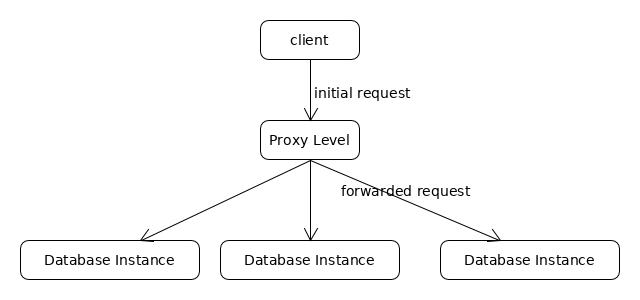
\includegraphics[scale=0.4]{images/abstract-database-arch.jpg}\hfill
This architecture may have several implementations:
\begin{itemize}
\item load balancer level - load balancer may include or implement this solution
\item hybrid: application level - it may be done as an own separate algorithm working on the top of request handling. 
\item manual redirection between nodes at the database level
\end{itemize}

Добавить общие понятия, load balancer, distributed hash table

We want to compare the architecture value of all of these solutions and propose the best one.
In the next section we consider load balancer level solution, in the section 2 - hybrid and in the section 3 - manual redirection at database level.

\chapter{Load balancer handling solution and its estimates}

Firstly let us remind what load balancer is.
From \cite{bib:brewer} load balancing is the technique that distributes the workload across multiple devices.
Generally it stands behind several web servers. It is most relevant to describe load balancer by the following scheme:

\centering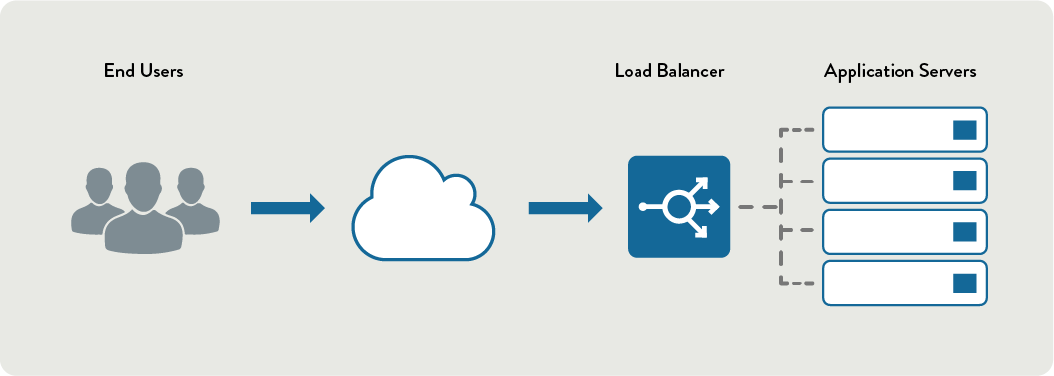
\includegraphics[scale=0.4]{images/application-delivery-load-balancing-diagram-simple-1.png}

Load balancer distributes traffic by different mechanisms. 


They are :
\begin{itemize}
\item[Round robin] default load balancing method. Round Robin mode passes each new connection request to the next server in line, eventually distributing connections evenly across the array of machines being load balanced.
\item[Weighted least]
\item[Ratio] The BIG-IP system distributes connections among pool members or nodes in a static rotation according to ratio weights that you define. In this case, the number of connections that each system receives over time is proportionate to the ratio weight you defined for each pool member or node. You set a ratio weight when you create each pool member or node.
\item[Dynamic Ratio] The Dynamic Ratio methods select a server based on various aspects of real-time server performance analysis. These methods are similar to the Ratio methods, except that with Dynamic Ratio methods, the ratio weights are system-generated, and the values of the ratio weights are not static. These methods are based on continuous monitoring of the servers, and the ratio weights are therefore continually changing
\item[Fastest (node) Fastest (application)] The Fastest methods select a server based on the least number of current sessions. 
\item[Least Connections ]The Least Connections methods are relatively simple in that the BIG-IP system passes a new connection to the pool member or node that has the least number of active connections.
.....
\end{itemize}


The way load balancer distributes traffic, lie on the hypothesis in the perfect way (see previous chapter).

Propose architecture (scheme).

Haproxy requires less additional feature to support our needs or even already implements them.

Consistent hashing algorithm or algorithm custom that takes list of available nodes from the request and load balance between them.

Focus on the state of the node.


The purpose of our load balancing technique is to redirect request to nodes that are already consistent making decision on the request.

Let's focus on dynamic ratio method.


Conclusion for this section: Nowadays there is lack of load balancers implementation that can support our need.
But a lot of them are opensource solutions and may be extended soon.


How many nodes at maximum load balancer supports
\chapter{Hybrid algorithm}
Other is described in next section (Algorithm)
\chapter{Own load balancing algorithm estimates}
Possibility to add it to load balancer
Where to get consistent nodes list from.

(Hash Table? masy be. another db? no. separate API? it anyway will take list from dynamic dict.)
so hash table to store nodes, its structure, evaluation of requests

\chapter{Distributed hash table}
What is distributed hash table and its implementations



The maximum size of hash table


Performance of different storages (redis, ...).


Formulas to keep it stably fast. 
Formula for number of nodes for DDS and number of keys in hash table (numbers of dataunits). 

Hash Table performance (read/write requests per second) - data from site, performance etc.


\chapter{Imitation model to communicate at load balancer level}
Architecture,  diagrams, or experiments with algorithm
sequence , activity diagrams for all three solutions.

To redirect over consistent nodes on API layer is a solution that delays response a lot.
Request come to not consistent node then redeirected to consistent node, but it is not alive,
then eventually come to the proper node. This solution is best to implement on load balancer algorithm level: get the consistent nodes and load balance between them by any enabled default  algorithm (round robin, least response time, ...)

But estimate both solutions.

Имитационная модель для КАЖДОГО из solutions.

\chapter{Mathematical Model of ... }
and model  to increase consistency value.


Let we have distributed datastore with such characteristics:
\begin{tabular*}{\textwidth}{cp{0.5cm}p{0.8\textwidth}}
$N$&& is a finite set of nodes of a distributed datastore; \\
$L$&& is a finite set of links of a distributed datastore; \\
$\partial:L\rightarrow 2^N$&& is a mapping that associates each link with two nodes that it binds;\\
$D$&& is a finite set of stored data units;\\
$r:D\rightarrow 2^N$&& is a mapping that associates each data unit $d$ with a subset of nodes 
that store its replica; \\

$N_d$&& is a finite set of nodes that are having given dataunit $d$; \\
$l(N_d)$&& is a number of nodes in datastore that are having given dataunit; \\
$n_c$&& is a number of nodes in a subset of $N_d$ where all nodes have the same replica.
\end{tabular*}
\chapter{Estimates, time complexity of algorithm basing on lb balancer, distributed hash table}
\chapter{Appendix: Load balancer, distributed hash table complexity estimates}
\begin{thebibliography}{00}

\bibitem{bib:prob_approach}
Kyrylo Rukkas, Galyna Zholtkevych:
Distributed Datastores: Towards Probabilistic Approach for Estimation of Dependability,
ICTERI 2015: 523-534


\bibitem{bib:lb}
P.P. Geethu Gopinatha, Shriram K.Vasudevan:
An In-depth Analysis and Study of Load Balancing Techniques in the Cloud Computing Environment, Procedia Computer Science Volume 50, 2015, Pages 427-432
https://www.sciencedirect.com/science/article/pii/S1877050915005104
https://devcentral.f5.com/articles/what-is-load-balancing-24740

\bibitem{bib:lb_mechanisms}

% https://help.utk.edu/kb/index2.php?func=show&e=1699

\end{thebibliography}
\end{document}
